\section{Summary}
\label{sec:Summary}

The scaling exponent $\eta_{Ising} = 0.25$ of the susceptibility on a $2D$ Ising lattice was examined with the Worm algorithm. This gave good results of $\eta = 0.26 \pm 0.002$.

Two different ways of determining the Hausdorff dimension of largest clusters at $T_c$ using the Worm algorithm was discussed. The scaling method examines the behaviour of the largest cluster as the system size increases. This gave the closest results to the geometrical Hausdorff dimension for a $2D$ Ising cluster of $D_H = 1.38 \pm 0.02$ compared to the analytical answer $D_H = 1.375$ \cite{Duplantier:GeoHausdorff}.

The second method was to approximate the Hausdorff dimension using the box dimension. This gave close results, $D_H = 1.35193 \pm 5 \cdot 10^{-4}$, to the scaling method but seem to diverge from the correct result for small boxes.

The resulting Hausdorff dimension of the 2D Ising lattice lies between the fractal dimension of a self avoiding walk with $D_{SAW} = 4/3$ \cite{Vilgis:FlorySAW}, and a pure random walk with $D_{RW} = 2$. This suggests a new type of self avoiding walk where `twisted loops' (see Section \ref{sec:Discussion}) can occur. A full comparison can be seen in Figure (\ref{fig:comparsion_2d_lattice_dimensions}).

The box counting method was then applied to a $3D$ XY lattice and gave the result $D_H = 1.77468 \pm 4 \cdot 10^{-6}$. This was then compared to previous results given by Hove, Mo and Sudbo as $D_H^S = 2.287 \pm 2 \cdot 10^{-3}$ \cite{Hove:hausdorff_crit_fluctuations}, and the result from the article disputing that claim by Prokof'ev and Svistunov with the value $D_H^P = 1.7655 \pm 2 \cdot 10^{-3}$ \cite{Prokofev:comment_on_hove_hausdorff_crit_fluct}. This strengthens the claim by Prokof'ev and Svistunov.

Due to time constraints the scaling method was not applied to the $3D$ XY model.

To simplify the simulations, the Villain approximation was used (See Section \ref{subsec:villainApprox}). The resulting new critical temperature was calculated by measuring the winding number on a range of temperatures. Since the winding number is proportional to the superfluid density, a sharp decrease can be seen around the critical temperature. By varying the system size, the intersections of all the drops can be taken as the critical temperature and was calculated to be $T_c = 0.3331 \pm 1 \cdot 10^{-4}$.

\section{Discussion}
\label{sec:Discussion}

The Worm algorithm is a good method for determining the Hausdorff dimension of a $2D$ Ising cluster. Scaling loop lengths gave the closest value $D_H = 1.38 \pm 0.02$ to the analytical answer $D_H = 1.375$\cite{Duplantier:GeoHausdorff}. This result could possibly be improved by more data as the analytical answer is within the error span.

Comparing the $2D$ Ising Hausdorff dimension to the fractal dimension of self avoiding walks, $D_{SAW} = 1.33$ \cite{Vilgis:FlorySAW}, and random walks, $D_{RW} = 2$, the Ising Worm algorithm produces something in between. As can be seen in Figure (\ref{fig:largest_cluster_illu}) the cluster ressembles a self avoiding walk but with `twisted loops' (See Figure (\ref{fig:twisted_loops})).

\begin{figure}[h!]
\centering
    \begin{subfigure}{.4\textwidth}
        \centering
        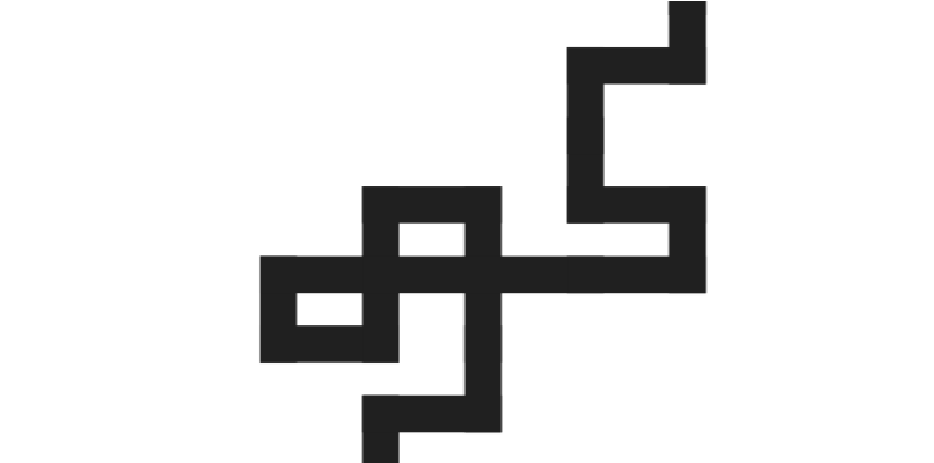
\includegraphics[width=\linewidth]{figures/twisted_loop1.pdf}
    \end{subfigure}
    \begin{subfigure}{.4\textwidth}
        \centering
        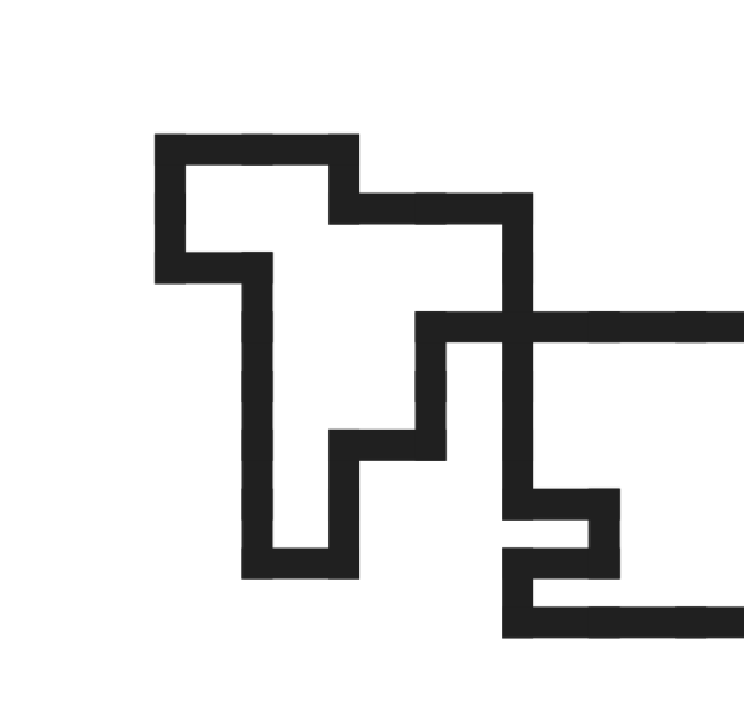
\includegraphics[width=\linewidth]{figures/twisted_loop2.pdf}
    \end{subfigure}
    \caption{Examples of twisted loops.}
\label{fig:twisted_loops}
\end{figure}

This implies that this may be a new type of self avoiding walk that may have similar properties.

In all simulations trying to measure the length of a loop, the choice was made that whenever there is ambiguity of which path to follow, all paths were followed. This avoids the technique of choosing a random path used by other articles \cite{Hove:hausdorff_crit_fluctuations}, and should in the average case return a longer loop. This can be intuitively understood by following the looping line in the number $8$. Whenever the crossing in the middle is reached, one has to follow one of the branching paths. If the stop condition is whenever the starting position is reached, there is a chance of only including one of the loops. This was avoided by recursively following all paths until all loops are explored.

The Hausdorff dimension of the $3D$ XY lattice heavily favoured the result of Prokof'ev and Svistunov over Hove, Mo and Sudbo with this thesis producing $D_H = 1.77468 \pm 4 \cdot 10^{-6}$ compared to theirs $D_H = 1.7655 \pm 2 \cdot 10^{-3}$ \cite{Prokofev:comment_on_hove_hausdorff_crit_fluct}. The result would have been strengthened by also comparing to the scaling method described in Section \ref{subsec:ScalingDimension}.

The winding number method provides a way of determining the critical temperature of a XY lattice. A weighted average of all intersections, weighted with the product of the linear system size of the two intersecting lines, was used to calculate the critical temperature. This method was chosen since the larger system was assumed to provide closer results to an infinite size system.

The choice to use the Hoshen Kopelman algorithm for cluster labeling (discussed in Section \ref{sec:HoshenKopelman}) reduced the simulation time considerably from the brute force methods used before. This together with a well chosen graph structure (discussed in Section \ref{subsec:LatticeImpl}) improved the data collection speed immensely.

All large scale simulations in this thesis were run on the Octopus cluster belonging to the department of theoretical physics at KTH.



